% Manuscript draft for JAMES: a differentiable global ocean model (Oceananigans + Reactant + Enzyme) and the
% stability of its adjoint. Build with `latexmk -pdf differentiable_ocean_manuscript.tex` in this directory.
% The structure follows the AGU template (Key Points, Abstract, Plain Language Summary, Open Research); the class
% is `article` until `agujournal2019.cls` is added. Text in \pending{...} waits on a result or a decision.
% Numbers come from the repository-root LOGBOOK.md (finding and job numbers in the comments).
\documentclass[11pt]{article}

\usepackage[margin=1in]{geometry}
\usepackage{amsmath, amssymb}
\usepackage{booktabs}
\usepackage{graphicx}
\usepackage{siunitx}
\usepackage{xcolor}
\usepackage[round]{natbib}
\usepackage{hyperref}
\usepackage{lineno}
\linenumbers

\newcommand{\gvec}{\mathbf{g}}
\newcommand{\xx}{\mathbf{x}}
\newcommand{\uu}{\mathbf{u}}
\newcommand{\pending}[1]{\textcolor{red}{[#1]}}
\newcommand{\sg}{\operatorname{sg}}

\title{A differentiable global ocean model on GPUs: exact adjoints, and why the linearized mesoscale closure is unstable}
\author{\pending{Authors and affiliations}}
\date{Draft of 21 November 2026}

\begin{document}
\maketitle

\section*{Key Points}
\begin{itemize}
  \item A GPU global ocean model with CATKE and GM/Redi closures is differentiated in reverse mode by Reactant
        and Enzyme, and verified.
  \item Compile time does not depend on the window: one step and its reverse pass are compiled once and driven by
        binomial checkpointing.
  \item The adjoint explodes through the derivative of the isopycnal slopes and, at 1 degree, of the WENO
        weights; fixing the buoyancy gradients in derivatives, and linear advection at 1 degree, bound it.
\end{itemize}

\begin{abstract}
We describe a differentiable configuration of a global ocean general circulation model that runs on graphics
processing units. The model is Oceananigans on a tripolar grid, with a split-explicit free surface, WENO advection,
the CATKE vertical mixing scheme and the Gent--McWilliams and Redi mesoscale closures. Reactant compiles one time
step of the model and Enzyme differentiates it in reverse mode. The host program drives the compiled step and its
reverse pass on a binomial checkpointing schedule, so the compile time (about 20 minutes) does not grow with the
length of the window. A gradient of the Atlantic overturning with respect to monthly surface fluxes then costs
3 minutes for 90 days and 10 minutes for a year at \ang{2} resolution on one GPU. Finite differences agree with the
adjoint to \numrange{e-9}{e-8} where the objective is smooth. Over windows of months the adjoint grows by one
e-fold per 17 hours and reaches \num{e23}, while twin forward experiments separate with an e-folding time of 12 to
15 days. We trace the growth to single near-surface cells in which one step of the linearized model amplifies a
perturbation 16 times. The amplification comes from the derivative of the isopycnal slopes in the mesoscale
closure, which scales with the inverse of the stratification. Holding the buoyancy gradients constant in
derivatives, with the forward model unchanged, reduces the one-step growth to 1.00 and bounds the 90-day adjoint
at \ang{2}. At \ang{1} a second instability appears, in the derivative of the WENO advection weights; with
linear upwind advection the \ang{1} 90-day adjoint is bounded as well. We show the resulting sensitivities of the
overturning at \ang{26.5}N to wind stress, heat flux and freshwater flux by lead time, and report what still
fails: the one-year window at \ang{2} has a further instability that these remedies do not remove.
\end{abstract}

\section*{Plain Language Summary}
Ocean models are usually run forward: given winds and heating, they predict currents. Many questions run the other
way: which winds, where and when, changed a current we care about? An adjoint model answers such a question in one
calculation, but writing one by hand takes years. Here the adjoint is generated automatically from the code of a
modern ocean model that runs on graphics cards. We check that the result is correct, and we measure its cost. We
also find that over a few months the adjoint blows up even though the ocean model itself is well behaved. The cause
is one formula, the slope of density surfaces, which is very sensitive where the ocean is weakly layered in winter.
Treating that slope as fixed when taking derivatives removes the blow-up for three-month calculations on a coarse
grid. On a finer grid a second formula, the weights of the advection scheme, has the same effect, and a simpler
advection scheme removes it. A one-year calculation still fails for reasons we have not yet found.

\section{Introduction}

The adjoint of an ocean general circulation model gives the gradient of one scalar, such as a transport or a
model--data misfit, with respect to all of the model's inputs in one backward integration. It is the basis of
ocean state estimation \citep{forget2015} and of sensitivity and attribution studies of the Atlantic meridional
overturning circulation (AMOC) \citep{marotzke1999, pillar2016, smith2019, kostov2021}. Nearly all of this work
rests on one model, the MITgcm, whose adjoint is generated by source-to-source automatic differentiation
\citep{giering1998, heimbach2005} of code written for that purpose.

Two developments make it worth revisiting how ocean adjoints are built. First, ocean models now run on graphics
processing units (GPUs) \citep{hafner2021, silvestri2025}, where a global simulation costs far less than on
processors. Second, automatic differentiation has moved into the compiler: Enzyme differentiates programs at the
level of the compiler's intermediate representation, including GPU kernels \citep{moses2020, moses2021}.
Differentiable programming is now proposed as a general foundation for Earth system models
\citep{gelbrecht2023}, and differentiable atmospheric models have been trained end to end \citep{kochkov2024}.
\citet{oceananigansenzyme} apply Enzyme and the compiler Reactant \citep{reactant} to four Earth system model
components written in Julia, Oceananigans among them. Their ocean application is an idealized re-entrant channel
on a rectilinear grid of $80\times160\times32$ cells, with no vertical mixing scheme, differentiated over 14 days
with square-root checkpointing inside the compiled program and checked against finite differences. The present
work extends that demonstration to a global configuration: a tripolar grid with realistic bathymetry, a
prognostic turbulence closure and mesoscale closures, forcing from reanalysis and state estimates, and windows of
months, where the stability of the adjoint becomes the limiting factor.

This paper makes three contributions.
\begin{enumerate}
  \item We differentiate a global configuration of Oceananigans \citep{ramadhan2020, wagner2025oceananigans} with
        realistic bathymetry, a tripolar grid, a turbulence closure with a prognostic equation \citep{wagner2025catke}
        and mesoscale closures \citep{gent1990, redi1982}, in reverse mode on a GPU, and verify the gradient against
        finite differences (Sections~\ref{sec:method} and~\ref{sec:verification}).
  \item We show that compiling one step and driving it from the host with binomial checkpointing
        \citep{griewank2000} makes the compile time independent of the window, and we give the costs
        (Section~\ref{sec:cost}).
  \item We find that the adjoint is unstable over months although the forward model is not, locate the instability
        in the derivative of the isopycnal slopes of the mesoscale closure, and show that holding the buoyancy
        gradients fixed in derivatives, as the MITgcm adjoint does, removes it for 90-day windows (Section~\ref{sec:stability}).
\end{enumerate}
Unstable adjoints are known from eddy-permitting models, where the linearization about a chaotic trajectory grows
without bound \citep{lea2000, kohl2002, hoteit2005}. The instability reported here is of a different kind. It occurs at
\ang{2} resolution, where the forward model is only weakly chaotic, and it belongs to a parameterization, not to
resolved dynamics. Approximating the adjoint of parameterizations is established practice, and the remedy we arrive at is not new.
In the ECCO version~4 adjoint the dependence of the vertical mixing coefficients on the ocean state is omitted,
and since 2008 the MITgcm adjoint has kept the mesoscale closure by ``omitting only the parametric dependency of
isopycnal slopes on the ocean density field'' together with a clipping of large slopes
\citep[their Section~4.2]{forget2015}. That choice is documented as a remedy but, to our knowledge, the instability
it removes has not been measured. Our contribution is the diagnosis in an adjoint generated by a compiler from
unmodified model code: the one-step amplification, where and when it occurs, and which term carries it.

Section~\ref{sec:model} describes the model, Section~\ref{sec:method} the differentiation,
Section~\ref{sec:verification} the verification and cost, Section~\ref{sec:stability} the instability, and
Section~\ref{sec:results} the AMOC sensitivities. Section~\ref{sec:limits} lists the limitations.

\section{Model and configuration}
\label{sec:model}

\subsection{Ocean model}

The model solves the hydrostatic Boussinesq equations with Oceananigans' \texttt{HydrostaticFreeSurfaceModel}
\citep{silvestri2025}, in the ocean-only configuration that NumericalEarth provides for the Ocean Model
Intercomparison Project \citep[OMIP;][]{griffies2016}. Table~\ref{tab:model} lists the settings.

\begin{table}[ht]
\centering\small
\begin{tabular}{@{}lp{0.74\textwidth}@{}}
\toprule
Grid & tripolar, $180\times60\times20$ (about \ang{2}) and $360\times180\times20$ (about \ang{1}); exponential
       vertical spacing to \SI{5500}{m}; fixed levels \\
Bathymetry & ETOPO, regridded and smoothed, minimum depth \SI{20}{m}; grid-fitted immersed boundary; Central
             American isthmus closed \\
Equation of state & TEOS-10 polynomial \citep{roquet2015} \\
Time stepping & split Runge--Kutta, third order, $\Delta t = \SI{2}{h}$ \\
Free surface & split-explicit \citep{shchepetkin2005}; 50 barotropic substeps at \ang{2}, 100 at \ang{1} \\
Advection & WENO, order 5 for momentum and 7 for tracers, explicit in the vertical \\
Vertical mixing & CATKE \citep{wagner2025catke}, with a latitude-dependent background diffusivity \\
Mesoscale closure & Gent--McWilliams skew flux and Redi diffusion \citep{gent1990, redi1982, griffies1998},
                    $\kappa = \SI{800}{m^2/s}$, slopes tapered above \num{e-2} \citep{danabasoglu1995} \\
Momentum closure & biharmonic viscosity with a 50-day damping time at the grid scale; implicit bottom drag \\
Precision & 64-bit floating point \\
\bottomrule
\end{tabular}
\caption{The forward model.}
\label{tab:model}
\end{table}

The configuration departs from the OMIP base configuration where differentiation or cost required it. The levels
are fixed instead of following the free surface. Vertical advection is explicit, because the adaptive implicit
scheme keeps state on the host. Shortwave radiation is absorbed at the surface. There is no sea ice, no river
runoff and no surface salinity restoring. Section~\ref{sec:limits} returns to these.

\subsection{Forcing and controls}

We use two forcings.
\begin{itemize}
  \item \emph{Bulk forcing.} The ocean starts at rest from a climatological state and is forced by the
        three-hourly JRA55-do atmosphere \citep{tsujino2018} through bulk formulae \citep{large2009}. The controls
        are the \SI{10}{m} winds on every atmosphere cell and forcing time, about \num{e8} numbers for 30 days.
        This forcing is used for verification.
  \item \emph{Prescribed fluxes.} The ocean starts from the ECCO version~4 state \citep{forget2015} of January
        1993 and is forced by ECCO's monthly wind stress, net heat flux and net freshwater flux, interpolated
        linearly in time. The controls are those four fields on every month, the controls of \citet{pillar2016}.
        This forcing is used for the sensitivity results.
\end{itemize}

\subsection{Objective}

The objective $J$ is the overturning streamfunction at \SI{1000}{m} across \ang{26.5}N in the Atlantic, the latitude
of the RAPID array \citep{mccarthy2015}. A row of the tripolar grid drifts from \ang{28}N to \ang{34}N across the
Atlantic, so the section is a staircase of cell faces that follows \ang{26.5}N from \ang{80}W to \ang{14}W. With
signed, wet-masked face areas $W^u$ and $W^v$ and the section area $a_k$ of level $k$,
\begin{equation}
T_k = \sum_{ij} \left(W^{v}_{ijk} v_{ijk} + W^{u}_{ijk} u_{ijk}\right), \qquad
\tilde T_k = T_k - \frac{\sum_{k'} T_{k'}}{\sum_{k'} a_{k'}}\, a_k, \qquad
J = -10^{-6} \sum_{k \le k_{\text{ref}}} \tilde T_k \quad [\si{Sv}],
\label{eq:objective}
\end{equation}
where levels are counted from the bottom and $k_{\text{ref}}$ is the level nearest \SI{1000}{m}. Removing the
section-mean velocity closes the streamfunction at the surface. $J$ is evaluated at the end of the window or
averaged over its last 30 days. It is linear in the velocities.

\section{Differentiation}
\label{sec:method}

\subsection{Compiling one step}

Reactant traces a Julia function into a tensor program and compiles it for the GPU. Enzyme differentiates that
program in reverse mode \citep{moses2020, moses2021}. We compile five functions once: the refresh of the model's
diagnostic state, one time step, and the reverse passes of the refresh, the step and the objective. A step maps the
model state and the controls to the next state, $\xx_n = \Phi(\xx_{n-1}; \uu)$. Its reverse pass maps the adjoint
of $\xx_n$ to the adjoint of $\xx_{n-1}$ and adds $(\partial\Phi/\partial\uu)^{\mathsf T}$ times that adjoint to
the gradient $\gvec = \partial J/\partial\uu$.

We arrived at this design after two others failed.
\begin{itemize}
  \item Differentiating a time loop of $N$ steps as one program did not fit in memory at two steps. Enzyme's
        reverse loop carried \num{64000} arrays (\SI{73}{GiB}) from one iteration to the next. Nearly all were
        gradients of intermediate values that are zero at every iteration boundary.
  \item Unrolling the $N$ steps into one program took \SI{48}{min} to compile at two steps, and the time grows
        with $N$.
\end{itemize}
Compiling one step has a further requirement. The state passed between steps must contain everything a step
reads: the prognostic fields alone are not enough, because a step uses tendencies and diffusivities computed at the
end of the previous one. A checkpoint is therefore a copy of every device array of the model except the grid and
the forcing.

\subsection{Checkpointing}

The reverse sweep needs the states $\xx_{N-1}, \dots, \xx_0$ in reverse order. The host stores a fixed number $c$ of
them and recomputes the others on the binomial schedule of \citet{griewank2000}, taken from Checkpointing.jl
\citep{schanen2023}. The 90-day window of 1080 steps uses $c = 40$. \pending{Number of forward steps recomputed.}
When $J$ is a time average, the adjoint receives the derivative of $J$ as an extra seed after each of the last
reverse steps. Because $J$ is linear, that seed does not depend on the state.

\subsection{Stop-gradients in the closures}
\label{sec:frozen}

Two options replace a quantity $q$ by $\sg(q)$, which has the value of $q$ and zero derivative. The forward model
is unchanged. The adjoint treats $q$ as given along the trajectory and omits the sensitivity that flows through it.
\begin{itemize}
  \item \emph{Frozen mixing}: $q$ is the set of viscosities and diffusivities that CATKE computes. ECCO
        version~4 makes the same approximation for its vertical mixing scheme \citep{forget2015}.
  \item \emph{Frozen buoyancy gradients}: $q$ is $(\partial_x b, \partial_y b, \partial_z b)$, stored once per
        refresh of the diagnostic state. The isopycnal slopes, their tapering and the stratification $N^2$ that the
        closures read are then constant in derivatives. The mesoscale fluxes are still differentiated with respect
        to the tracers they transport. This is the approximation of the MITgcm adjoint \citep{forget2015},
        without its change of tapering scheme in the forward model.
\end{itemize}
Storing the buoyancy gradients changes the order of operations in one place. CATKE's turbulent kinetic energy is
stepped after the tracers of a stage and before the refresh, so with stored gradients it read the $N^2$ of the
previous stage, and $J$ after 90 days changed by a fraction \num{1.1e-4}. We refresh the stored gradients before
that step. The forward models with stored and with inline gradients then agree to rounding: \num{4e-16} in
temperature after one step on a processor, and \num{2e-6} in $J$ after 90 days on a GPU. Section~\ref{sec:stability}
gives the reason for the second option.

\section{Verification and cost}
\label{sec:verification}

\subsection{Finite differences}

Let $d = \gvec/\lVert\gvec\rVert$. We compare $\gvec^{\mathsf T}d$ with finite differences of $J$ along $d$ over 25
octaves of the step $h$, at 8, 84 and 360 time steps (16 hours, one week and 30 days) with the bulk forcing
(Figure~\ref{fig:fd}). Where $J$ is smooth the central difference agrees with the adjoint to \numrange{4e-9}{2e-8}.
The compiled forward model was also compared with the same model run without Reactant on a processor: $J$ agrees
to \num{7.5e-13} after one step and \num{2.2e-15} after two.

\begin{figure}[ht]
\centering
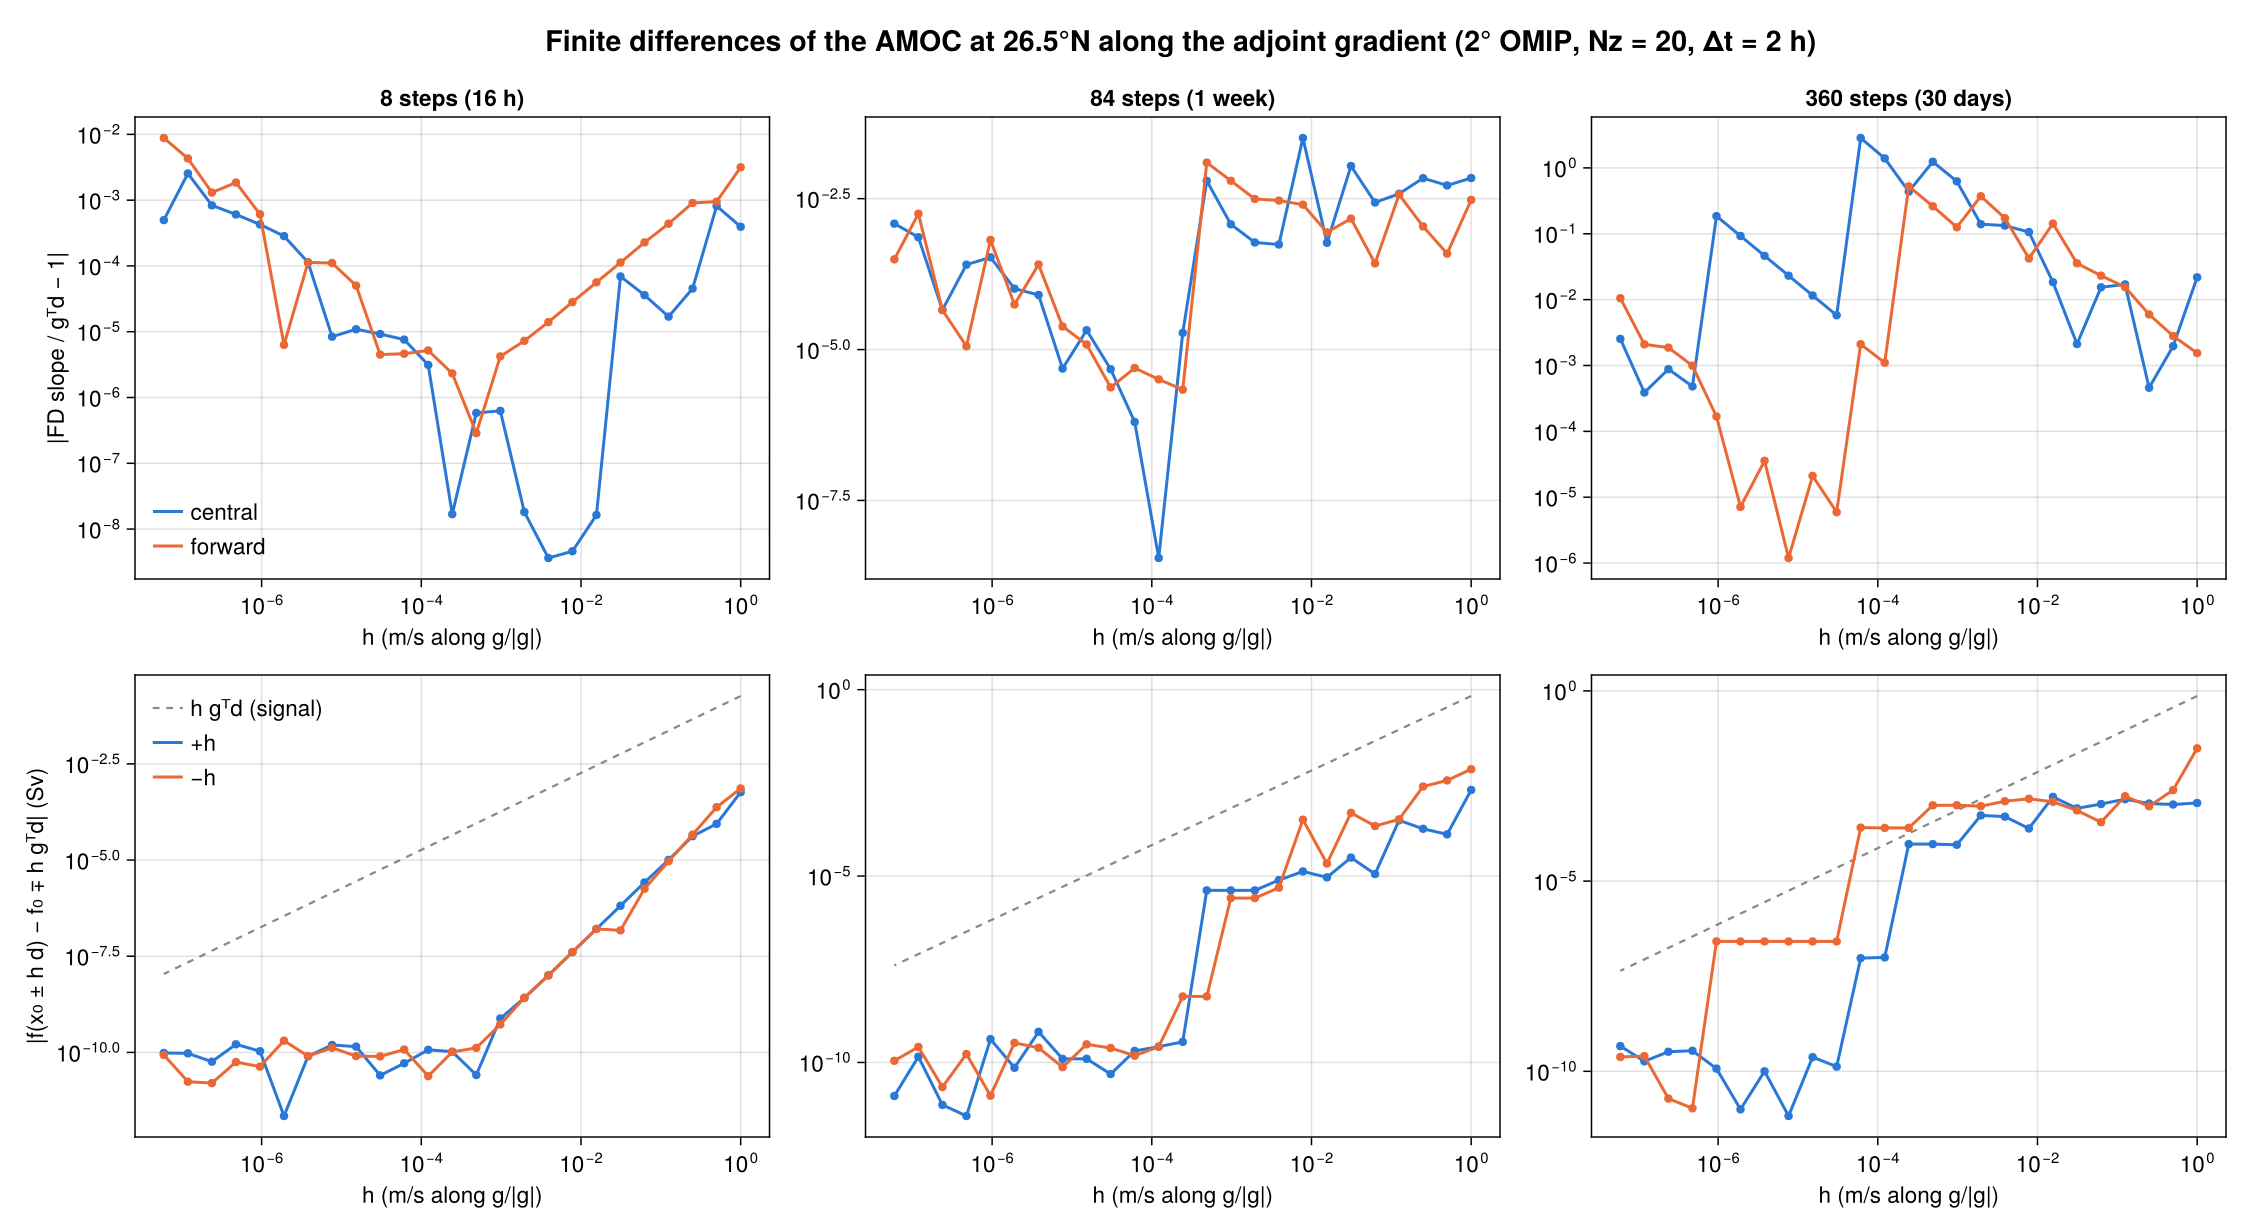
\includegraphics[width=0.8\textwidth]{figures/fd_scans_twodegree_nz20.png}
\caption{Finite differences of $J$ along $d = \gvec/\lVert\gvec\rVert$ at 8, 84 and 360 steps. Top: error of the
central and forward differences relative to $\gvec^{\mathsf T}d$. Bottom: residual of the linear prediction on each
side of the base state, with the signal $h\,\gvec^{\mathsf T}d$ dashed. A residual that stays constant as $h$
shrinks is a jump in $J$.}
\label{fig:fd}
\end{figure}

Beyond about a day $J$ is only piecewise smooth. Perturbations above a threshold make $J$ jump by
\SIrange{e-7}{e-3}{Sv}, and the residual of the linear prediction stops falling with $h$. The threshold shrinks
with the window: no jumps occur at 8 steps for $h \le \SI{1}{m/s}$, and at one week $J$ is smooth only for
$h \le \SI{2.4e-4}{m/s}$. The adjoint differentiates the branch that the forward run took, as in
\citet{lea2000}. A Taylor test with small $h$ therefore fails on a long window even when the gradient is correct,
and a gradient must be judged at an amplitude where the jumps are small beside the signal. At $h$ between 0.25 and
\SI{1}{m/s} the secant slope matches $\gvec^{\mathsf T}d$ to \num{4e-4} at 8 steps, \numrange{5e-3}{7e-3} at one
week and \numrange{5e-4}{2e-2} at 30 days. \pending{Identify the switches: CATKE's convective and stable branches
are the likely source but this is not confirmed.}

These scans used Oceananigans 0.113.5. On the release used for the results below (0.117.2) the gradient passes
Taylor tests at 2 steps with the bulk forcing and at 8 steps with prescribed fluxes
(relative error \numrange{5e-6}{9e-6}). Changing the Reactant version changed the 8-step gradient by
\num{1.7e-12} (stress) and \num{5e-10} (heat and freshwater fluxes).

\subsection{Stop-gradients}

With frozen mixing the gradient is no longer exact, and the measure of its quality is the secant at finite
amplitude. At one week and at 30 days the frozen-mixing gradient has cosine 0.9996 and 0.994 with the full
gradient, and predicts the finite-amplitude response 0.4 to \SI{1.7}{\percent} less accurately. Integrals of the
gradient that cancel are less robust: the response to a uniform meridional wind at 30 days is
\SI{0.76}{Sv} per m/s with frozen mixing and \SI{0.32}{Sv} per m/s without. Over 90 days with prescribed fluxes
the frozen-mixing gradient predicted secants along its own direction to \SI{2.2}{\percent} (Oceananigans 0.113.5).
With frozen buoyancy gradients as well (Oceananigans 0.117.2), the 90-day gradient predicts secants along the
direction of the wind-stress gradient to \SIrange{0.2}{0.6}{\percent}: the secant slopes at
$h = 0.1$, 0.05 and \SI{0.025}{N.m^{-2}} are 18.93, 18.94 and \SI{18.87}{Sv} per \si{N.m^{-2}}, and
$\gvec^{\mathsf T}d$ is 18.82. The secants do not converge monotonically, as expected of a piecewise-smooth $J$,
so the agreement cannot be tightened by reducing $h$.

\subsection{Cost}
\label{sec:cost}

\begin{table}[ht]
\centering\small
\begin{tabular}{@{}lrrrr@{}}
\toprule
Window & Checkpoints & Compile & First gradient & Later gradients \\
\midrule
\multicolumn{5}{@{}l}{Bulk forcing, \ang{2}, A100, Reactant 0.2.303} \\
2 steps (4 h) & 1 & \SI{27.1}{min} & \SI{2368}{s} & \SI{0.82}{s} \\
8 steps (16 h) & 3 & \SI{28.4}{min} & \SI{2350}{s} & \SI{3.5}{s} \\
84 steps (1 week) & 12 & \SI{27.3}{min} & \SI{2241}{s} & \SI{28}{s} \\
360 steps (30 days) & 30 & \SI{29.1}{min} & \SI{2367}{s} & \SI{104}{s} \\
\midrule
\multicolumn{5}{@{}l}{Prescribed fluxes, \ang{2}, GH200, Reactant 0.2.309} \\
1080 steps (90 days) & 40 & \SI{17}{min} & \SI{183}{s} & \SI{183}{s} \\
4380 steps (1 year) & \pending{c} & \SI{17}{min} & \SI{599}{s} & \SI{599}{s} \\
\bottomrule
\end{tabular}
\caption{Cost of a gradient on one GPU. The forward model alone takes \pending{time} for 90 days.}
\label{tab:cost}
\end{table}

Table~\ref{tab:cost} gives the costs. The compile time does not depend on the window. With Reactant 0.2.303 the
first gradient spent about \SI{39}{min} on the host before the first step ran; Reactant 0.2.309 removed that
cost. A 90-day gradient at \ang{2} then takes \SI{3}{min} and a one-year gradient \SI{10}{min}. At \ang{1} one
reverse step makes a single allocation of \SI{31.8}{GiB}, so those runs need a GPU with \SI{80}{GB} or more.
At \ang{1} the compile takes \SI{16.6}{min} and a 90-day reverse sweep \SI{9.7}{min}, against \SI{3.1}{min} for
the forward model alone.

\section{Stability of the adjoint}
\label{sec:stability}

\subsection{The adjoint grows; the forward model does not}

With frozen mixing, the adjoint of windows longer than one to three months grows backward in time by about one
e-fold per \SI{17}{h}, and the gradient reaches \numrange{e13}{e23} or is not finite. On Oceananigans 0.117.2 the
90-day window from January 1993 gives $J = \SI{17.91}{Sv}$ and a largest stress sensitivity of \num{e23} Sv per
N m$^{-2}$, where values of order one are expected.

None of the following changes to the model bounded the one-year adjoint: halving the time step, linear third-order
upwind advection in place of WENO, Laplacian or biharmonic lateral tracer diffusion, convective adjustment,
Laplacian viscosity of up to \SI{5e4}{m^2/s}, and a window ending in a different season. A diffusion applied only in
the reverse pass (verified by a dot-product test) reduced the 90-day growth by a factor of 17, far from enough.

The forward model does not have this growth. We ran pairs of forward integrations of the same compiled step that
differ by noise of \SI{e-6}{K} in temperature. Over 60 days the root-mean-square difference grew by factors of 60
and 110 for two start dates, an e-folding time of 12 to 15 days. Noise of \SI{e-3}{K} grew by less than 10.
Single cells did change by a factor of 100 within three days. The forward map is therefore steep in places but
bounded, and the growth of the adjoint is a property of the linearization. Damping can only hide it.

\subsection{Where and when the adjoint grows}

We recorded the largest adjoint of each prognostic field, and its location, once per model day during the reverse
sweep. The adjoint does not grow steadily. It stays near \num{2e4} and then rises by several decades per day in
short bursts. In the 90-day window the first burst is at the separation of the Kuroshio
(\ang{146}E \ang{39}N) and the second at the Grand Banks (\ang{49}W \ang{43}N), both near the surface in winter and
both led by the adjoint of salinity. With upwind advection the bursts occur at the same two places, so the
advection scheme is not the cause (Figure~\ref{fig:trace}).

\begin{figure}[ht]
\centering
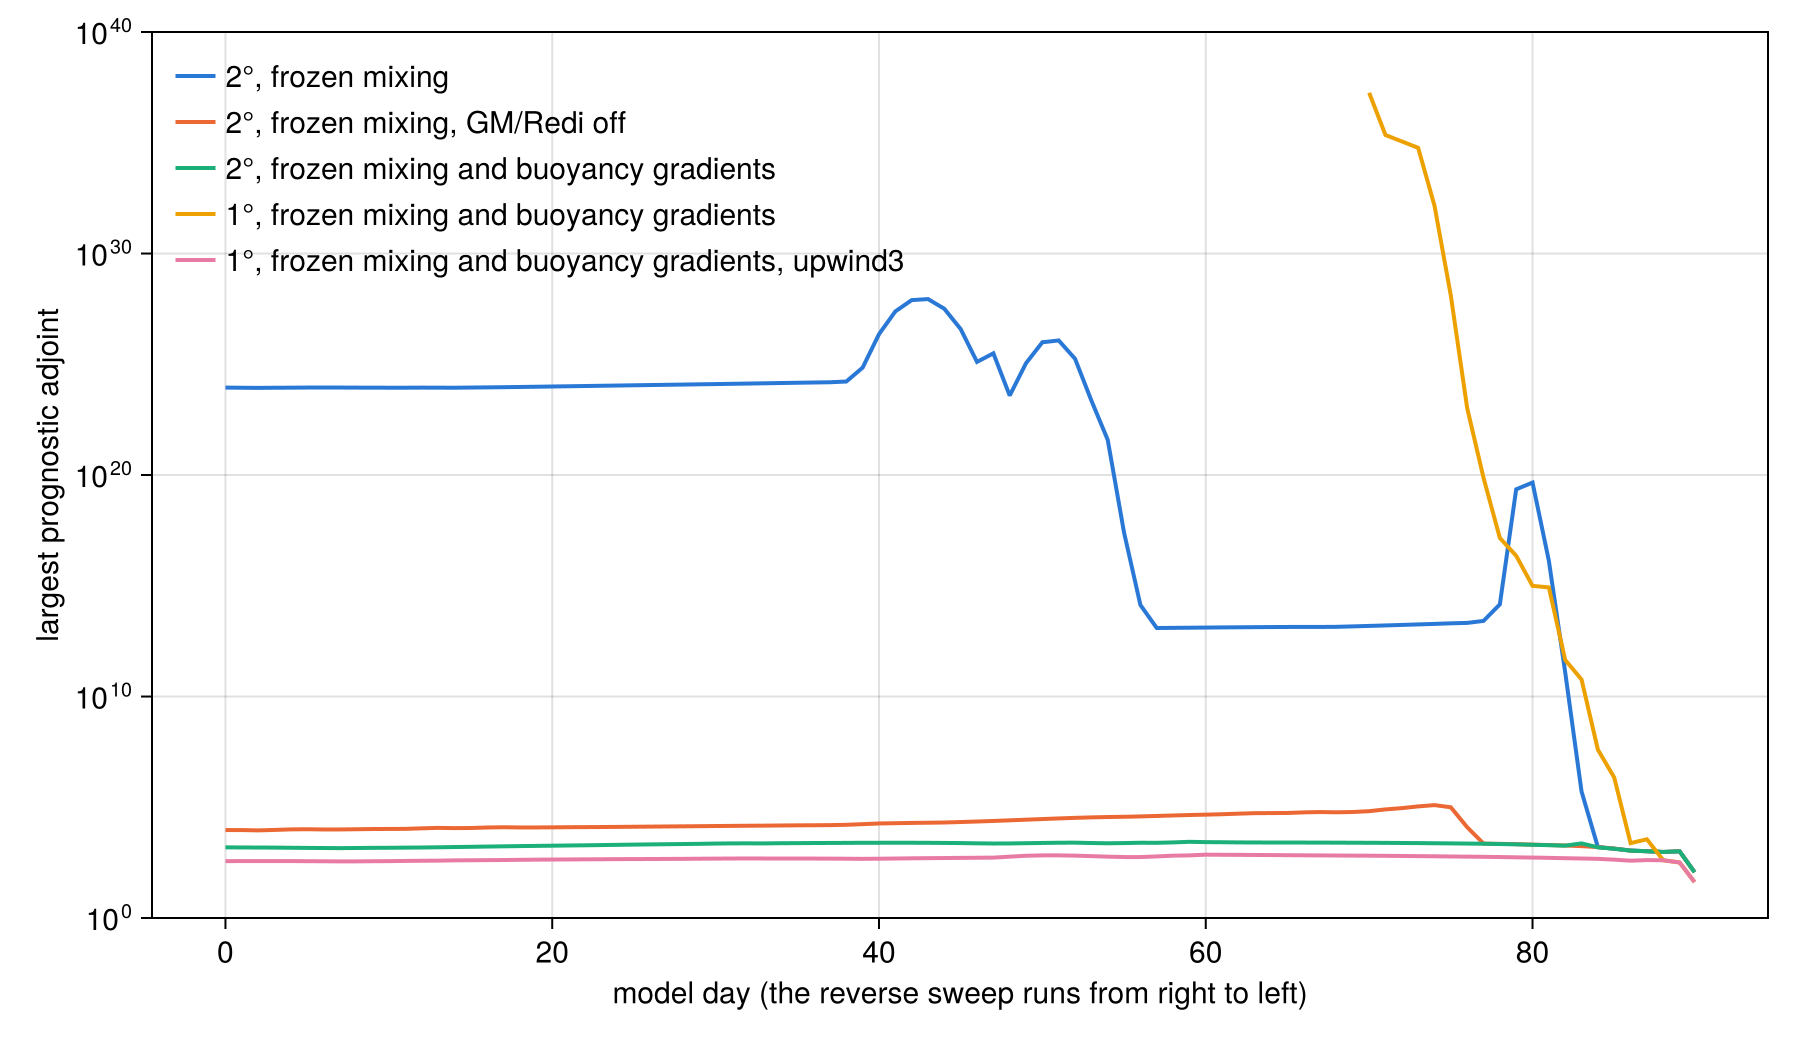
\includegraphics[width=0.8\textwidth]{figures/adjoint_trace_ecco4_nz20_oc117.png}
\caption{Largest adjoint of the prognostic fields (velocities, temperature, salinity and free surface) at each
model day of the reverse sweep of the 90-day window, which runs from day 90 to day 0. A curve ends where the adjoint
overflows. All runs use WENO advection except the last, which uses linear third-order upwind advection.}
\label{fig:trace}
\end{figure}

\subsection{One step of the linearized model}

To separate the instability of one step from growth along the trajectory, we fix the state at a step inside a
burst and apply the reverse pass of that step repeatedly, renormalizing each time. This power iteration converges
to the largest eigenvalue of the step's Jacobian $\partial\Phi/\partial\xx$ at that state. Table~\ref{tab:jacobian}
gives the result at two states of the 90-day window.

\begin{table}[ht]
\centering\small
\begin{tabular}{@{}lrr@{}}
\toprule
& State at day 81.5 & State at day 87 \\
\midrule
Frozen mixing & 16.2 & 3.99 \\
Frozen mixing, no mesoscale closure & 1.21 & 1.30 \\
Frozen mixing and frozen buoyancy gradients & 1.00 & 0.99 \\
\bottomrule
\end{tabular}
\caption{Growth per \SI{2}{h} step of the leading mode of one step's reverse pass, by power iteration (60
iterations, converged after about 10).}
\label{tab:jacobian}
\end{table}

A factor of 16.2 per step is more than 14 decades per day. Each mode occupies a single cell about \SI{60}{m} below the
surface, one in the Barents Sea and one at the Grand Banks, where the adjoint of the vertical component of the
Redi diffusion tensor is largest. The forward (tangent-linear) derivative of the step has the same eigenvalue, so
the instability belongs to the linearized step and not to the reverse-mode transformation. Without the mesoscale
closure the growth falls to 1.2--1.3 per step and the 90-day adjoint is bounded (largest stress sensitivity 2.7).

\subsection{Interpretation: the derivative of the slope}

The mesoscale closure transports tracers along and across isopycnals with fluxes that depend on the slope
\begin{equation}
\mathbf{S} = -\frac{\nabla_h b}{\partial_z b},
\qquad
\frac{\partial \mathbf{S}}{\partial(\partial_z b)} = \frac{\nabla_h b}{(\partial_z b)^2} = -\frac{\mathbf{S}}{N^2}.
\label{eq:slope}
\end{equation}
The vertical Redi flux is proportional to $\kappa\,|\mathbf{S}|^2\,\partial_z c$ for a tracer $c$. The forward
model bounds that term by tapering the slope. Its derivative with respect to the stratification is not bounded in
the same way. Where $N^2$ is small the slope is
large, tapering switches on, and a small change in temperature or salinity changes the flux by a large factor.
Since $b$ depends on the tracers that the flux transports, the linearized step contains a feedback from a tracer
perturbation to its own tendency through $\mathbf{S}$, with a gain that scales with $1/N^2$. This is consistent
with where the modes sit (near-surface cells in winter) and with salinity leading them.
\pending{This is an interpretation. To confirm it: evaluate the terms of Equation~\ref{eq:slope} in the two cells,
or freeze the slope and the tapering factor separately.}

Frozen mixing does not remove this term, because it holds CATKE's diffusivities fixed but still differentiates the
slopes. Freezing the buoyancy gradients (Section~\ref{sec:frozen}) removes it: the one-step growth is 1.00 and 0.99
(Table~\ref{tab:jacobian}).

\subsection{The 90-day adjoint with frozen buoyancy gradients}

With both options the 90-day adjoint is bounded. The adjoint of the prognostic fields stays below \num{2.8e3}
throughout the reverse sweep, and the largest stress sensitivity is \num{3.9} Sv per N m$^{-2}$
(Figure~\ref{fig:growth}). $J$ is unchanged to \num{2e-6}.

\begin{figure}[ht]
\centering
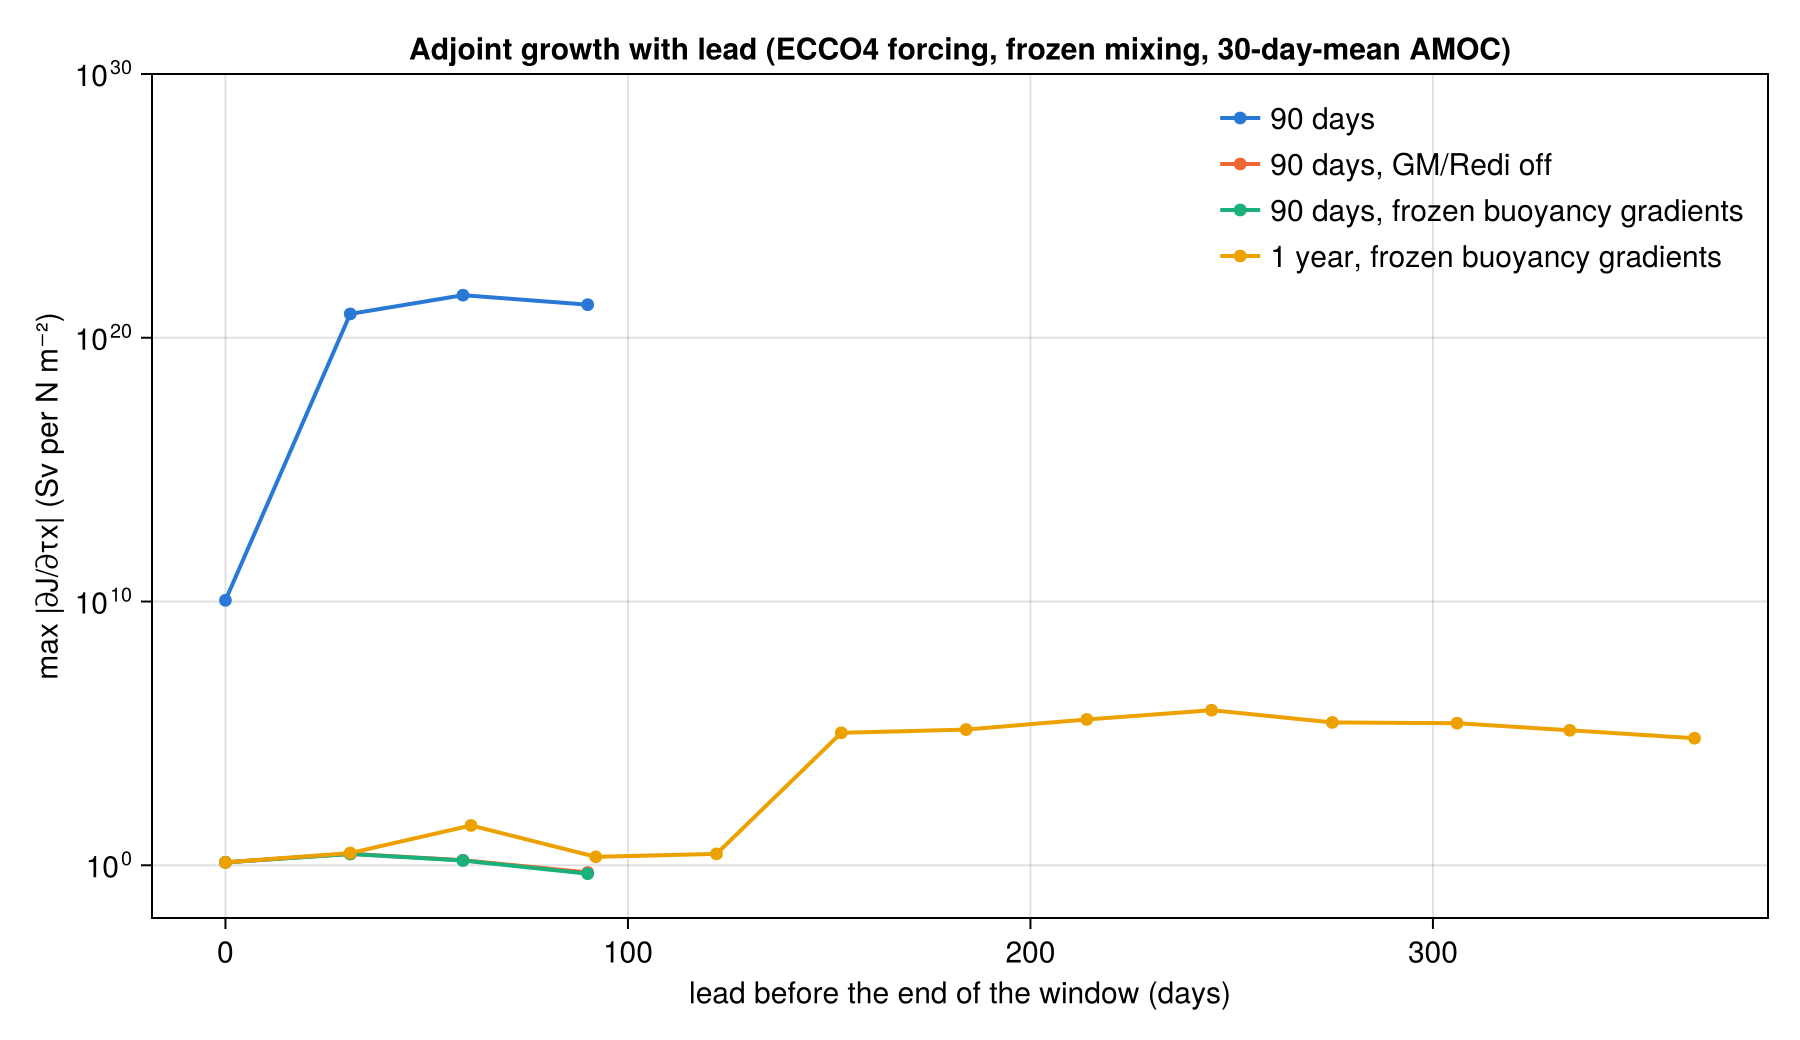
\includegraphics[width=0.7\textwidth]{figures/lead_growth_ecco4_nz20_oc117.png}
\caption{Largest sensitivity of $J$ to the zonal wind stress over cells, for each monthly forcing field, against
lead time. All runs use frozen mixing. The curve without the mesoscale closure lies under the curve with frozen
buoyancy gradients.}
\label{fig:growth}
\end{figure}

\subsection{One degree}

At \ang{1} the forward model needs a shorter barotropic step: with 50 substeps per \SI{2}{h} step it is not finite
after one day, and with 100 it runs the 90 days ($J = \SI{16.36}{Sv}$). The adjoint of that window, with frozen
mixing and frozen buoyancy gradients, is not bounded (Figure~\ref{fig:trace}). It stays below \num{4e3} for five
days of the reverse sweep, then grows by two to five decades per day and overflows after 21 days. The growth
occurs in three groups of cells in the southwest Indian Ocean: the Mozambique Channel (\ang{36}E \ang{26}S, near
the surface), the Agulhas Return Current (\ang{45}E \ang{41}S, at mid-depth) and north of Madagascar
(\ang{51}E \ang{11}S). None of these is a site of the \ang{2} bursts.

The one-step Jacobian shows that this is a different instability from the one at \ang{2}. At two states inside the
first bursts (days 83.5 and 85.5) the leading growth is 23.7 and 19.2 per step with frozen buoyancy gradients, and
10.3 and 6.5 per step without the mesoscale closure, where the same test at \ang{2} gave 1.0 and 1.2 to 1.3. In all
four cases the mode sits in the horizontal velocities, with 87 to \SI{90}{\percent} of its energy in a
$3\times3\times3$ box of cells at mid-depth; the mode at day 85.5 with frozen buoyancy gradients is at the Agulhas
Return Current site of the sweep (\ang{45}E \ang{42}S). Neither the mesoscale closure nor the buoyancy gradients
carry this growth.

The advection scheme does. With linear third-order upwind advection of momentum and tracers in place of WENO, and
frozen buoyancy gradients, the leading growth at the same two model days is 0.99 per step, and the mode is spread
over the domain (the largest $3\times3\times3$ box holds under \SI{1}{\percent} of its energy). WENO's weights
depend on the advected field, and their derivative enters the linearized step; a linear scheme has none. The
growth is not an effect of the step length: at $\Delta t = \SI{1}{h}$ with WENO it is 2.9 and 4.7 per step, that
is 8.5 and 22 per \SI{2}{h}. Each variant follows its own forward trajectory, so these compare model days and not
states.

With linear upwind advection the \ang{1} 90-day adjoint is bounded (Figure~\ref{fig:trace}). With frozen mixing and
frozen buoyancy gradients its largest prognostic value stays between \num{4e1} and \num{7.2e2} over the whole
sweep, led by the adjoint of salinity in the subtropical North Atlantic near the objective's section (\ang{17}W to
\ang{78}W, \ang{11}N to \ang{35}N), and the largest sensitivity to wind stress is \SI{1.2}{Sv} per \si{N.m^{-2}}.
The forward model changes with the scheme: $J$ is \SI{14.51}{Sv} with upwind advection and \SI{16.36}{Sv} with WENO.
\pending{Why WENO's weights are benign at \ang{2}, where the sweep with WENO and frozen buoyancy gradients is
bounded; and whether the weights can be held constant in derivatives, as the buoyancy gradients are, so that the
forward model keeps WENO.}

\subsection{One year}

With frozen buoyancy gradients the one-year gradient is finite, where every earlier one-year run was not finite or
exceeded \num{e13}. It is not usable. From the end of the year back to day 242 the adjoint stays below \num{7e3}.
Around day 204 the adjoint of salinity grows from \num{1.8e5} to \num{2.7e11} within two days in one column west
of the Antarctic Peninsula (\ang{63}W \ang{61}S), at \SIrange{1.1}{1.7}{km} depth. It stays near \num{e9} in that
column for the rest of the sweep, and the gradient with respect to the earlier forcing fields reaches
\num{7.6e5} Sv per N m$^{-2}$. This second instability is deep, not near the surface, and we have not identified
the term. \pending{One-step Jacobian at the day-204 burst.}

\section{Sensitivity of the overturning at \ang{26.5}N}
\label{sec:results}

Figure~\ref{fig:lead} shows the sensitivity of the AMOC averaged over days 61 to 90 to each monthly forcing
field, after Figure~1 of \citet{pillar2016}, with frozen mixing and frozen buoyancy gradients at \ang{2}.

\begin{figure}[ht]
\centering
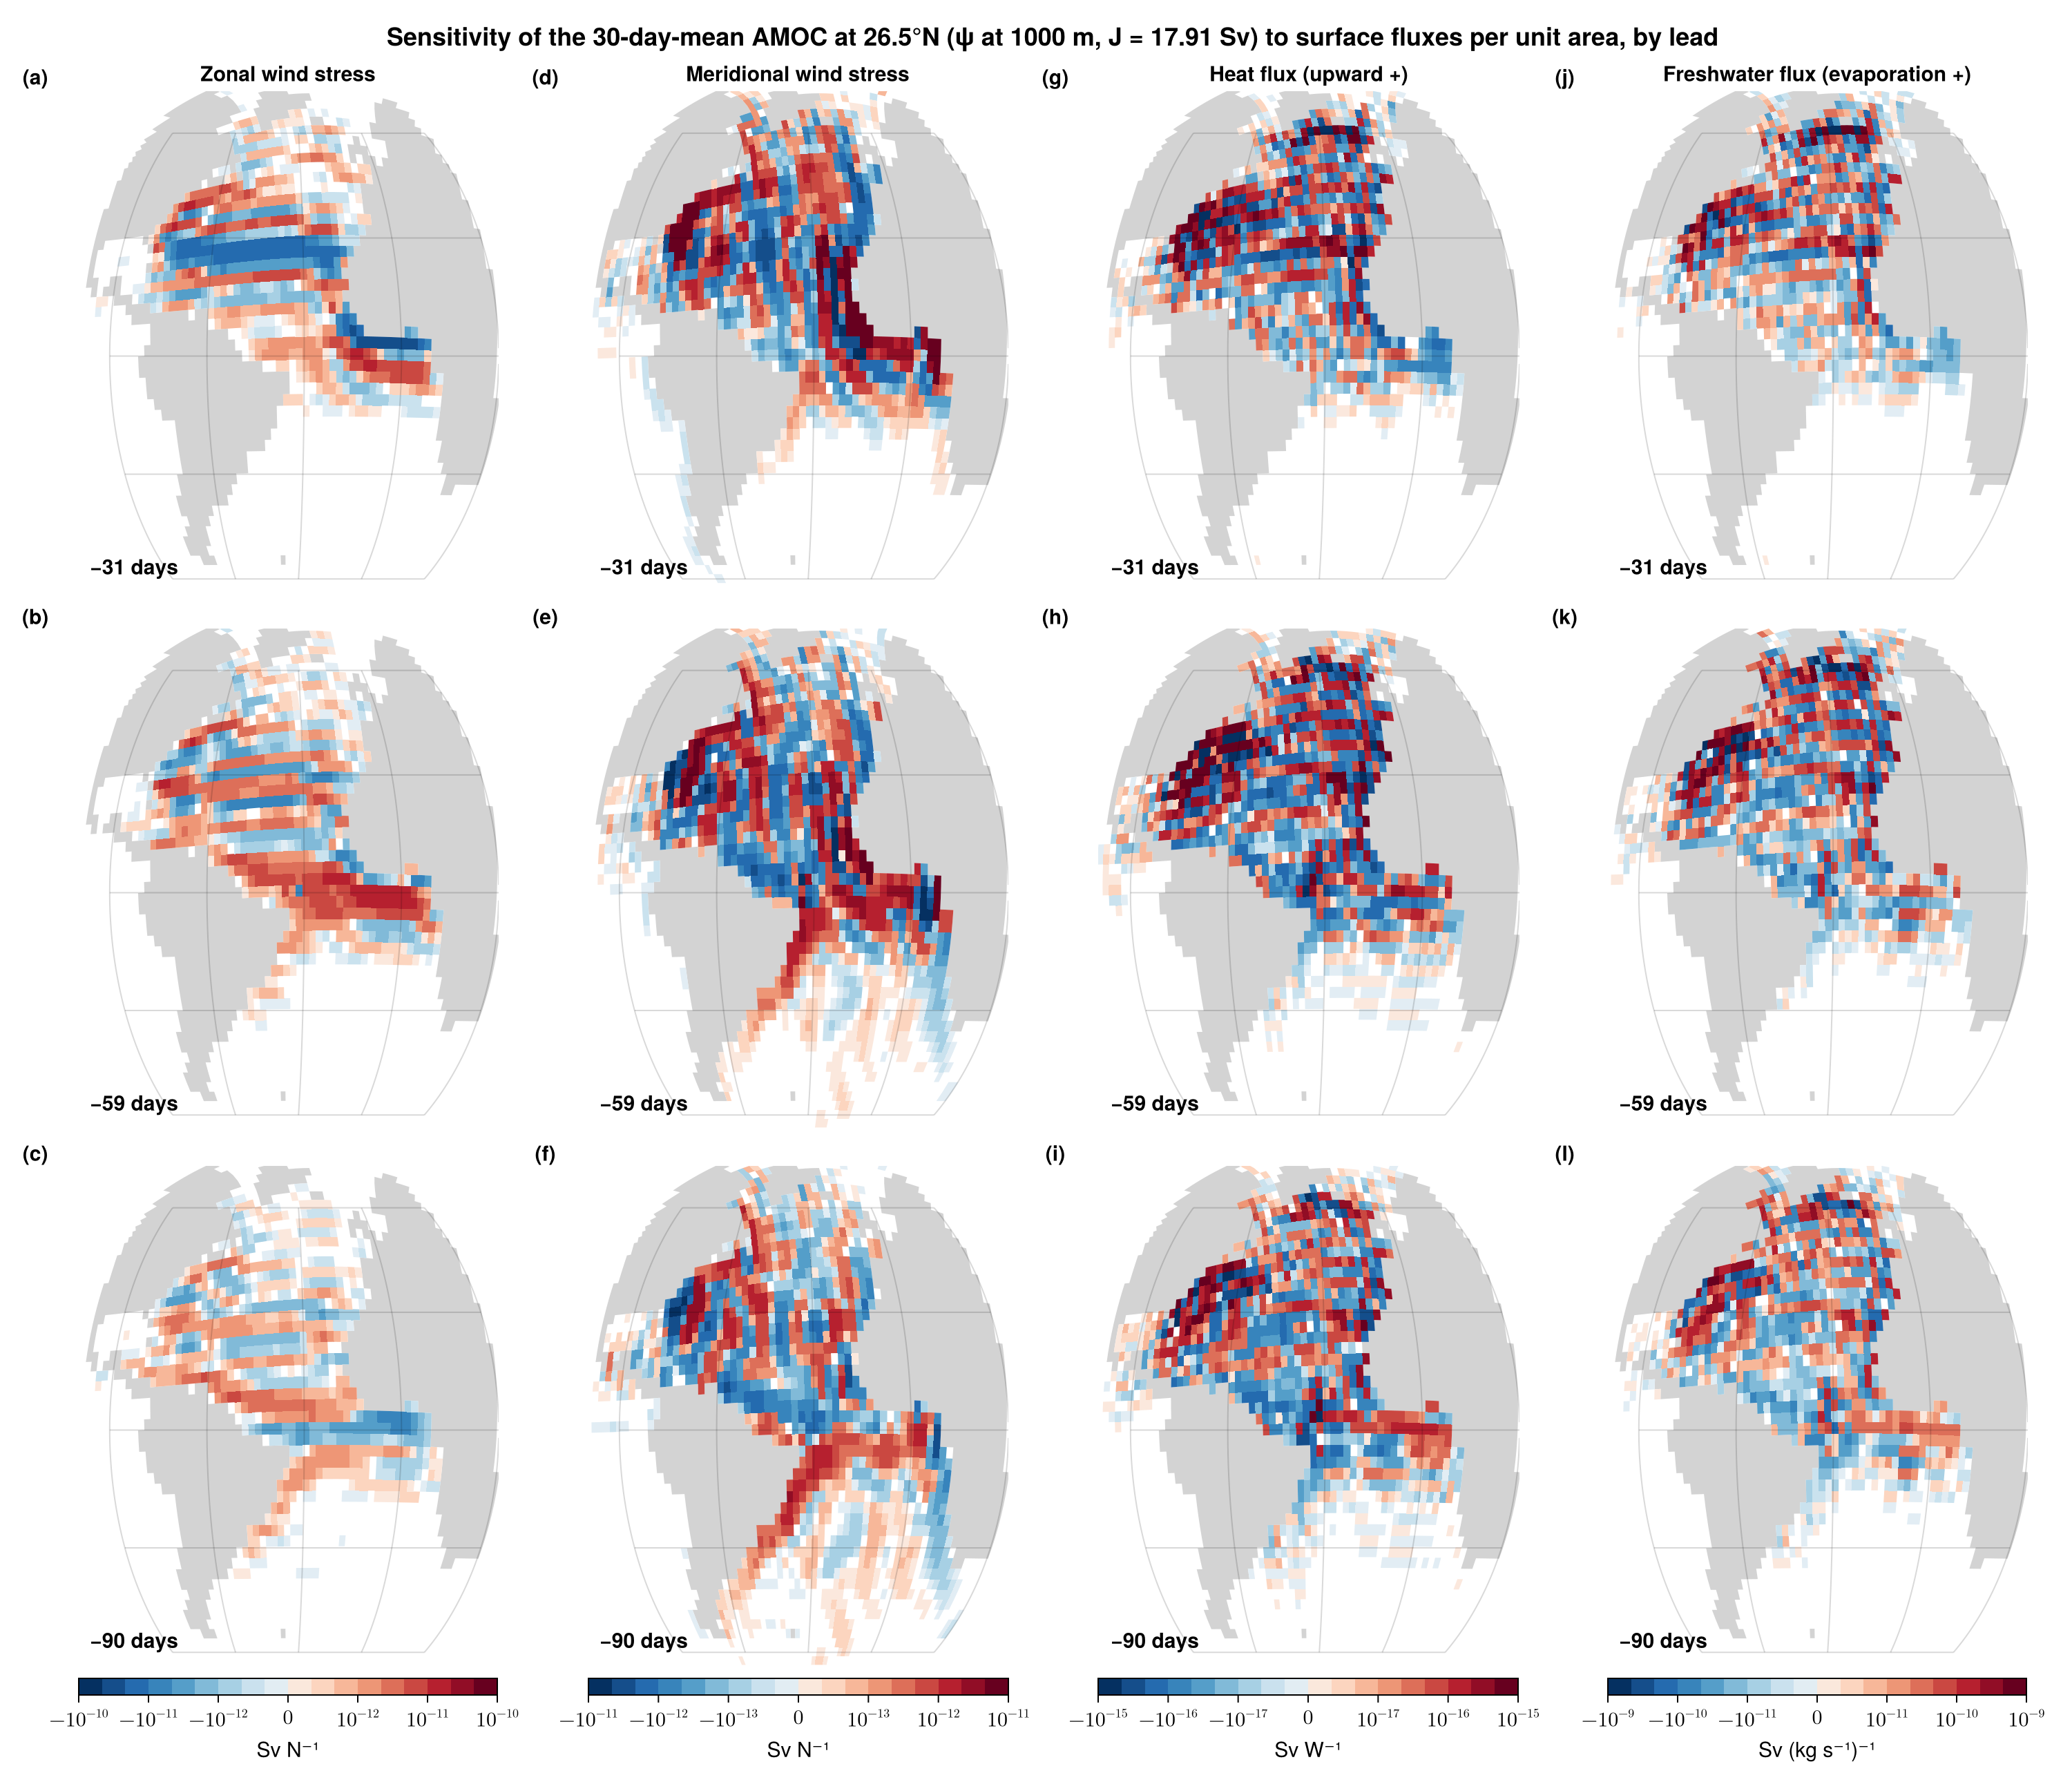
\includegraphics[width=0.85\textwidth]{figures/lead_sensitivity_ecco4_nz20_90day_frozen_gradients.png}
\caption{Sensitivity of the 30-day-mean AMOC at \ang{26.5}N ($J = \SI{17.91}{Sv}$) to each monthly flux field, per
unit area, by lead time (rows) and forcing (columns). Upward heat flux and evaporation are positive. Colors are
logarithmic over three decades.}
\label{fig:lead}
\end{figure}

At a lead of one month the sensitivity to zonal stress lies in zonal bands at and north of the section, the local
Ekman response. The sensitivity to meridional stress lies along the western boundary, the African coast and the
equator, and spreads into the tropics and the South Atlantic at longer leads. These are the pathways of
\citet{pillar2016} at leads of one and three months. \pending{Quantitative comparison with Pillar et al., if their
fields are available.}

The stress sensitivities are robust to the change of model version: against Oceananigans 0.113.5 with frozen mixing
only, the cosine per monthly field is 0.98 to 0.999 and the maxima agree to \SI{1}{\percent}. The heat and
freshwater flux sensitivities are less robust (cosine 0.76 to 0.90) and show a checkerboard at the grid scale. We
do not interpret them.

We do not yet show sensitivities at \ang{1}: the bounded \ang{1} adjoint uses upwind advection, whose forward
state differs from the WENO configuration of this section. \pending{\ang{1} sensitivities with upwind advection,
or with WENO and frozen weights.}

\section{Limitations and outlook}
\label{sec:limits}

\begin{itemize}
  \item \emph{The frozen adjoint is an approximation.} It omits the sensitivity that acts through changes in
        vertical mixing and in isopycnal slopes. For frozen mixing we measured the cost in accuracy
        (Section~\ref{sec:verification}); with frozen buoyancy gradients the 90-day gradient matches secants
        along its own direction to under \SI{1}{\percent}, which does not test other directions.
  \item \emph{One year is out of reach, and \ang{1} needs a different advection scheme.} A further instability
        remains in the one-year window (Section~\ref{sec:stability}). At \ang{1} the adjoint is bounded only with
        linear upwind advection, which changes the forward model. Each bounded result may not survive a change of
        resolution, season or model version.
  \item \emph{The initial states are not in equilibrium.} The windows start from rest or from the ECCO state
        interpolated to a different grid, and the model adjusts during the window.
  \item \emph{The configuration is simplified}: no sea ice, no surface restoring, fixed levels, explicit vertical
        advection, 20 levels.
  \item \emph{Why the newer model version is less stable is not known.} The same 90-day window was bounded with
        frozen mixing alone on Oceananigans 0.113.5.
\end{itemize}
The stop-gradient on the buoyancy gradients is a blunt remedy. A slope computation whose derivative is bounded,
for example a regularized stratification in the denominator of Equation~\ref{eq:slope}, would keep the
sensitivity that acts through the slopes and would also change the forward model. Whether that is preferable
depends on the application.

\section*{Open Research}
The model, the adjoint package, the configuration files of every run and the plotting scripts are in the
NumericalEarth.jl repository \pending{URL, branch, and an archived release with a DOI}. The software versions are
Oceananigans 0.117.2, Reactant 0.2.309, Enzyme 0.13.216 and Julia 1.12.7. \pending{Data: ECCO version 4 and
JRA55-do access statements.}

\section*{Acknowledgments}
\pending{Funding, computing allocation (Texas Advanced Computing Center), and people.}

\appendix
\section{Compiler issues}
\label{sec:compiler}

Differentiating a model of this size exposed problems in the compiler stack. We list them because they determined
the design of Section~\ref{sec:method}, and because the fixes are in the versions we name.
\begin{itemize}
  \item \emph{Zero-valued loop state.} The reverse of a time loop carried \SI{73}{GiB} of arrays that are zero at
        every iteration boundary. Fixed in Enzyme-JAX (\#3971).
  \item \emph{Slow rewrite patterns.} Two patterns of the optimizer cost tens of minutes on the differentiated
        program. One is fixed upstream (\#3970); we exclude the other.
  \item \emph{First call.} With Reactant 0.2.303 the first call of each compiled function spent 13 to
        \SI{40}{min} on the host. Reactant 0.2.309 removed this.
  \item \emph{Tripolar fold.} A wrong adjoint at the fold of the tripolar grid was fixed in Oceananigans
        (\#6396).
  \item \emph{Julia 1.13.} The first compile does not finish within \SI{3.8}{h}; the runs use Julia 1.12.
\end{itemize}

\bibliographystyle{plainnat}
\bibliography{differentiable_ocean}

\end{document}
